\section{Proposed Approach}

The proposed scheme operates as a three-stage pipeline, as illustrated in Fig.~\ref{fig:scheme}. A consensus protocol processes neighborhood state information to produce an error vector $\mathbf{z} = [a, \alpha]^T$, which feeds the exponential control law to generate a reference velocity $\mathbf{u}_\text{ref} = [v, \omega]^T$. This reference is then passed to the Feasible Velocities Polygon module, which incorporates LiDAR measurements to enforce collision avoidance and outputs the admissible command $\mathbf{u}^*$.

\begin{figure}[h]
    \centering
    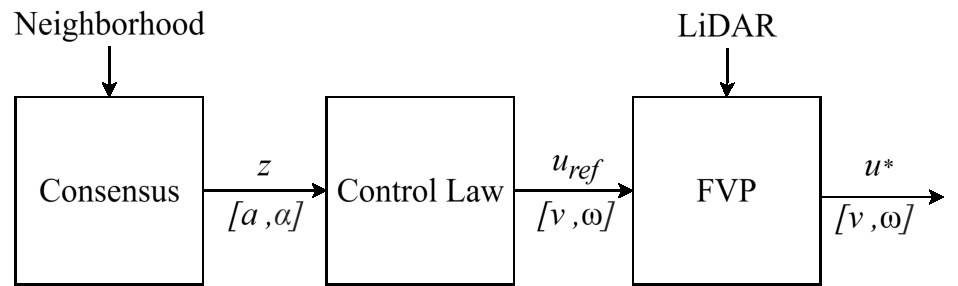
\includegraphics[width=1.0\linewidth]{Pics/esquema2.drawio.pdf}
    \caption{Block diagram of the proposed control scheme. The consensus module processes neighborhood information and produces the error vector $\mathbf{z} = [a, \alpha]^T$, which drives the exponential control law to generate a reference velocity $\mathbf{u}_\text{ref}$. The FVP module incorporates LiDAR measurements to enforce collision avoidance and outputs the admissible command $\mathbf{u}^*$.}
    \label{fig:scheme}
\end{figure}

\subsection{Graph-Theoretic Communication Models}

Let $\mathcal{S} = \{1, \ldots, n\}$ be the set of $n$ differential-drive robots. The communication structure of the system is modeled as a directed graph $\mathcal{G}(t) = (\mathcal{S}, \mathcal{E}(t))$, where $\mathcal{E}(t) \subseteq \mathcal{S} \times \mathcal{S}$ is the set of active edges at time $t$. A pair $(j, i) \in \mathcal{E}(t)$ indicates that agent $i$ receives information from agent $j$ at instant $t$. The neighborhood of agent $i$ is defined as:

\begin{equation}
    \mathcal{N}_i(t) = \{ j \in \mathcal{S} : (j,i) \in \mathcal{E}(t) \}
    \label{eq:neighbors}
\end{equation}

The weighted adjacency matrix $\mathcal{A} = [a_{ij}] \in \mathbb{R}^{n \times n}$ is defined as $a_{ij} > 0$ if $(j,i) \in \mathcal{E}(t)$ and $a_{ij} = 0$ otherwise, with $a_{ii} = 0$. The associated Laplacian matrix $\mathcal{L} = [l_{ij}] \in \mathbb{R}^{n \times n}$ is defined as:

\begin{equation}
    l_{ij} =
    \begin{cases}
        \sum_{k \neq i} a_{ik} & \text{if } i = j \\
        -a_{ij} & \text{if } i \neq j
    \end{cases}
    \label{eq:laplacian}
\end{equation}

To guarantee convergence of the consensus protocol, $\mathcal{G}(t)$ must contain a directed spanning tree, a necessary and sufficient condition for $\mathcal{L}$ to have exactly one zero eigenvalue~\cite{ren2006consensus,mesbahi2010graph}. The communication topology is updated dynamically according to:

\begin{equation}
    (j,i) \in \mathcal{E}(t) \iff \| \mathbf{p}_i(t) - \mathbf{p}_j(t) \| \leq r_c
    \label{eq:topology}
\end{equation}

\noindent where $r_c > 0$ is the communication radius and $\mathbf{p}_i = [x_i\ y_i]^T$ is the position of agent $i$ in the plane.

\subsection{Kinematic Model}

The multi-agent system is composed of $n$ differential-drive robots, each modeled as a unicycle system. For agent $i \in \mathcal{S}$, the kinematic model is:

\begin{equation}
    \dot{\mathbf{q}}_i = \mathbf{J}(\mathbf{q}_i)\mathbf{u}_i =
    \begin{bmatrix}
        \cos\theta_i & 0 \\
        \sin\theta_i & 0 \\
        0 & 1
    \end{bmatrix}
    \begin{bmatrix}
        v_i \\ \omega_i
    \end{bmatrix}
    \label{eq:unicycle_multi}
\end{equation}

\noindent where $\mathbf{q}_i = [x_i\ y_i\ \theta_i]^T \in \mathbb{R}^2 \times \mathbb{S}^1$ is the configuration vector and $\mathbf{u}_i = [v_i\ \omega_i]^T$ the control input, subject to:

\begin{equation}
    |v_i| \leq v_{\max}, \quad |\omega_i| \leq \omega_{\max}
    \label{eq:vel_limits}
\end{equation}

The non-holonomic constraint of each agent is implicitly preserved in the structure of $\mathbf{J}(\mathbf{q}_i)$, which prevents instantaneous lateral displacement. The control law~\eqref{eq:control_law} generates trajectories that simultaneously correct position and orientation, converging exponentially toward the desired reference, as illustrated in Fig.~\ref{fig:trajectory}.

\begin{figure}[h]
    \centering
    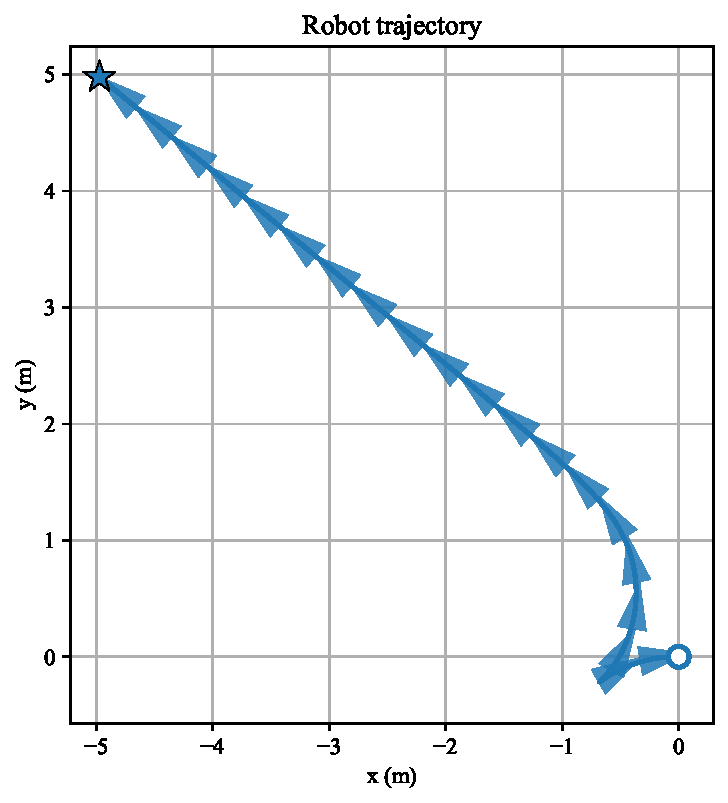
\includegraphics[width=0.8\linewidth]{Pics/trajectory.pdf}
    \caption{Trajectory generated by the exponential control law for a differential-drive robot navigating from point $A$ to point $B$. The curve reflects the simultaneous correction of position and orientation characteristic of the unicycle model under non-holonomic constraints.}
    \label{fig:trajectory}
\end{figure}

\subsection{Consensus Protocol and Formation Strategy}

An error-based consensus protocol is proposed to provide the input variables of the control law defined in~\eqref{eq:control_law}. Since this law operates on a distance $a_i$ and a relative angle $\alpha_i$, the consensus error of agent $i$ is defined as the weighted average of position differences with respect to its active neighbors:

\begin{equation}
    \mathbf{e}_i =
    \begin{bmatrix} e_x \\ e_y \end{bmatrix}
    = \frac{1}{|\mathcal{N}_i|}
    \sum_{j \in \mathcal{N}_i} a_{ij}(t)
    \begin{bmatrix} x_j - x_i \\ y_j - y_i \end{bmatrix}
    \label{eq:consensus_error}
\end{equation}

\noindent where $|\mathcal{N}_i|$ denotes the cardinality of the neighborhood of agent $i$. From this error vector, the variables required by the control law are obtained:

\begin{equation}
    a_i = \sqrt{e_x^2 + e_y^2}
    \label{eq:consensus_a}
\end{equation}

\begin{equation}
    \alpha_i = \text{atan2}(e_y,\, e_x) - \theta_i
    \label{eq:consensus_alpha}
\end{equation}

The reference velocities for each follower are obtained by substituting~\eqref{eq:consensus_a} and~\eqref{eq:consensus_alpha} into~\eqref{eq:control_law}:

\begin{equation}
    \mathbf{u}_{i,\text{ref}} =
    \begin{bmatrix} v_{i,\text{ref}} \\ \omega_{i,\text{ref}} \end{bmatrix}
    =
    \begin{bmatrix} k_1\, a_i \cos\alpha_i \\ k_2\, \alpha_i + k_1 \sin\alpha_i \cos\alpha_i \end{bmatrix}
    \label{eq:ref_velocity}
\end{equation}

For leader-following with formation maintenance, an offset $\boldsymbol{\psi}_i = [\psi_i^x\ \psi_i^y]^T \in \mathbb{R}^2$ is defined for each follower $i \in \mathcal{S}$, representing its desired position relative to the leader. Based on the consensus protocol proposed in~\cite{koulong2024distributed}, the following modification is introduced: rather than applying consensus on raw positions, the protocol operates on the offset-shifted positions $(\mathbf{x}_i - \mathbf{r}_i)$, ensuring that the desired formation is an exact equilibrium point. The state of each follower evolves as:

\begin{equation}
    \dot{\mathbf{x}}_i = -\sum_{j \in \mathcal{N}_i} a_{ij}\left[(\mathbf{x}_i - \mathbf{r}_i) - (\mathbf{x}_j - \mathbf{r}_j)\right] - \beta\, b_i^0\left(\mathbf{x}_i - \mathbf{x}_0 - \mathbf{r}_i\right)
    \label{eq:formation_error}
\end{equation}

\noindent where $b_i^0 \in \{0,1\}$ indicates whether agent $i$ has direct communication with the leader and $\beta > 0$ is the attraction gain. At equilibrium, $\mathbf{x}_i = \mathbf{x}_0 + \mathbf{r}_i$ for all $i \in \mathcal{S}$, and the consensus term vanishes identically. The protocol objective is to guarantee:

\begin{equation}
    \lim_{t \to \infty} \left[ \mathbf{p}_i(t) - \mathbf{p}_0(t) - \mathbf{r}_i \right] = \mathbf{0}, \quad \forall\, i \in \mathcal{S}
    \label{eq:formation_objective}
\end{equation}

\noindent The proposed protocol induces in each robot a reference velocity $\mathbf{u}_{i,\text{ref}}$ consistent with its non-holonomic dynamics, which is subsequently filtered by $\text{FVP}_i$ to guarantee inter-agent collision avoidance.

\subsection{Anisotropic Collision Avoidance}

For agent $i \in \mathcal{S}$, the environment is perceived through a LiDAR sensor whose frame is displaced from the robot frame by the vector $\mathbf{r}_p = [r_p\ 0]^T \in \mathbb{R}^2$, with displacement only along axis $X_{r_i}$. 

The sensor provides a set of measurements $\mathcal{O}_i = \{(d_{ik}, \phi_{ik})\}$, where $d_{ik}$ is the distance to the point detected by ray $k$ and $\phi_{ik}$ is its angle in the robot frame. The influence zone is bounded by $d_{\iota} > 0$, so that only measurements with $0 < d_{ik} \leq d_{\iota}$ generate active constraints.

Each active measurement is mapped as a linear constraint in the velocity space $(v_i, \omega_i)$ through the velocity damper model~\cite{ramirez2001collision}:

\begin{equation}
    A_{ik}\, v_i + B_{ik}\, \omega_i \leq C_{ik}
    \label{eq:lidar_constraint}
\end{equation}

\noindent where the coefficients are obtained from the rigid-body kinematics of the robot-sensor system:

\begin{equation}
    \begin{aligned}
        A_{ik} &= -\cos(\phi_{ik}), \\
        B_{ik} &= -\|\mathbf{r}_p\|\sin(\phi_{ik}), \\
        C_{ik} &= -\xi\,\frac{d_{ik} - d_s}{d_{\iota} - d_s}
    \end{aligned}
    \label{eq:coefficients}
\end{equation}

\noindent with $d_s > 0$ the safety distance and $\xi > 0$ a convergence coefficient. The term $B_{ik} = \|\mathbf{r}_p\|\sin(\phi_{ik})$ captures the rotational contribution of $\omega_i$ evaluated at the sensor mounting point, resulting from applying rigid-body kinematics to vector $\mathbf{r}_p$~\cite{ramirez2001collision}. The set of constraints~\eqref{eq:lidar_constraint} together with the velocity limits~\eqref{eq:vel_limits} defines the Feasible Velocities Polygon of agent $i$:

\begin{equation}
    \text{FVP}_i = \left\{ \mathbf{u}_i \in \mathbb{R}^2 \,\middle|\,
    \begin{aligned}
        &A_{ik} v_i + B_{ik} \omega_i \geq C_{ik},\ \forall k \in \mathcal{O}_i \\
        &|v_i| \leq v_{\max},\ |\omega_i| \leq \omega_{\max}
    \end{aligned}
    \right\}
    \label{eq:fvp}
\end{equation}

The admissible control vector $\mathbf{u}_i^* = (v_i^*, \omega_i^*)$ is obtained as the projection of the reference velocity $\mathbf{u}_{i,\text{ref}}$ onto $\text{FVP}_i$:

\begin{equation}
    \mathbf{u}_i^* = \arg\min_{\mathbf{u}_i \in \text{FVP}_i} \frac{1}{2} \| \mathbf{u}_i - \mathbf{u}_{i,\text{ref}} \|^2
    \label{eq:projection}
\end{equation}

\noindent This formulation is inherently anisotropic, as each constraint depends on the angle $\phi_{ik}$ of the detected ray with respect to the robot frame, capturing the directional nature of the non-holonomic system in its interaction with neighboring agents.